\begin{figure*}[t]\centering
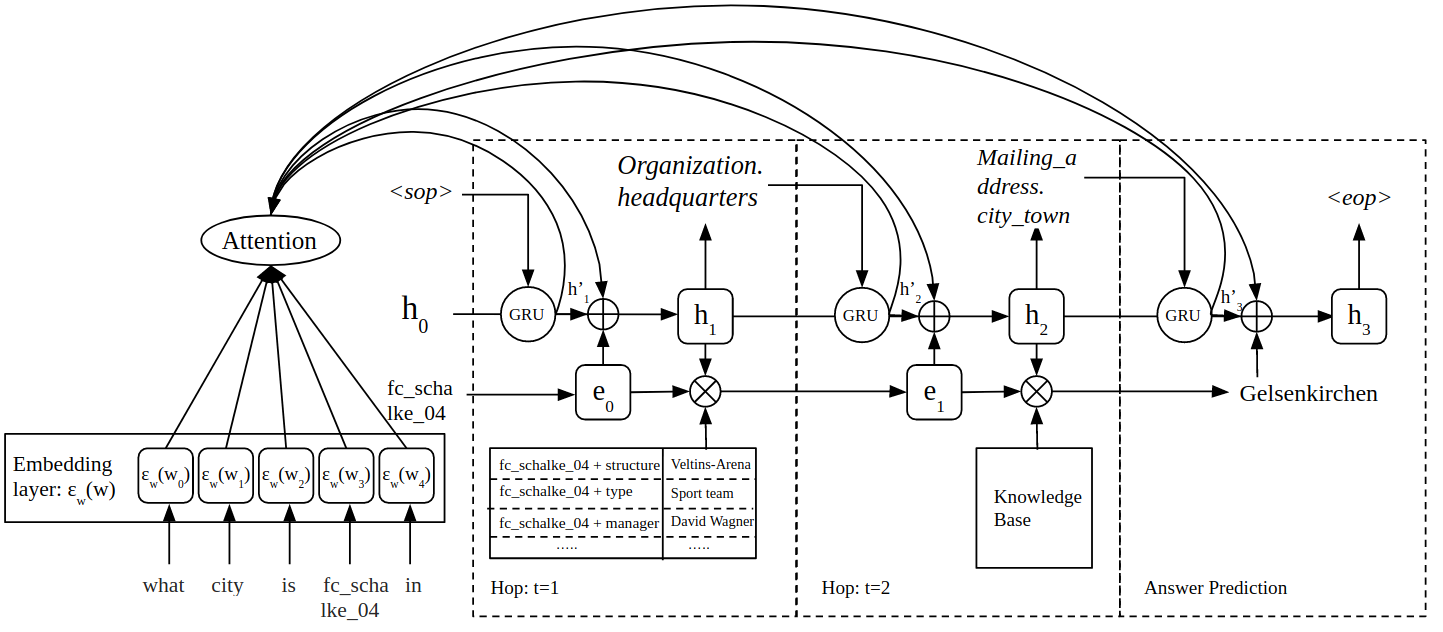
\includegraphics[width=2.0\columnwidth]{figs/model.png}
\caption{\fontsize{10}{12}\selectfont An illustration of how our model works with a QA pair \textit{"What city is fc\_schalke\_04 in?"} and \textit{Gelesenkirchen}. The entity linker extracts \textit{fc\_schalke\_04} as the topic entity. We only show one possible paths here: $r_1$ is \textit{Organization.headquarters} and $r_2$ is \textit{Mailing\_address.city\_town}, our model can be used to output the probability of this given path. The symbol $\bigoplus$ represents concatenation, and $\bigotimes$ represents knowledge base lookup. }
\label{fig:model}
\end{figure*}


\section{Model}
We first introduce some notations. For a given question $q$ and its topic entity $e_0$ (identified by entity linking tool), a reasoning path is a sequence in the form $\mathbf{p} = (e_0, r_{1},e_{1},r_{2}, \cdots,e_{T-1}, r_{T})$ that points to the answer entity $e_T=y$. That is, $\mathbf{p}\rightarrow e_T=y$. Each step $(e_{t-1},r_t,e_t)$ is a valid fact in the knowledge base $\mathcal{KB}$. Our goal is to build a model that can use multiple paths $\mathbf{p}$ to predict answer $y$ given question $q$ and topic entity $e_0$. In this section, we first present the design of our model architecture, and then explain the training and inference algorithms in detail. 

\subsection{Model Architecture}


%Figure \ref{fig:model} illustrates the architecture of our model. All the words $w_0,w_1,\cdots,w_{|q|-1}$ in the given question $q$ are first sent to a fixed embedding layer to acquire word embeddings $\varepsilon_w(w_0),\varepsilon_w(w_1),\cdots,\varepsilon_w(w_{|q|-1})$. \cheng{Does the symbol match the one in diagram?} To reduce computational cost, the embedding layer is pre-trained and not updated during training. %The word embeddings are combined in different ways based on attention weights to show different reasoning focus at each hop.
% $\varepsilon(\cdot)$ function represents gathering embedding of the input from the corresponding pre-trained embeddings matrix. 



%\subsubsection{Reasoning Decoding} The decoding module consists of relation prediction module and entity prediction module.


Figure \ref{fig:model} illustrates the architecture of our model. We model path probability using recurrent neural network with gated recurrent units (GRU). At a timestep $t$, the input hidden representations of GRU unit and predicted relation are denoted by $h_{t-1}$ and $r_t$ respectively. The model relies on the attention mechanism~\cite{DBLP:journals/corr/BahdanauCB14} to produce a question context vector $c_t$. Specifically, all the words $w_0,w_1,\cdots,w_{|q|-1}$ in the given question $q$ are first sent to a fixed embedding layer to acquire word embeddings $\varepsilon_w(w_0),\varepsilon_w(w_1),\cdots,\varepsilon_w(w_{|q|-1})$. Next we apply GRU to produce a temporary hidden state $h_{t}'=GRU(h_{t-1}, r_{t-1})$, and then apply a parameterized feed-forward neural network $a$ to calculate the similarity score $u_{tk} = a(h'_{t},\varepsilon_w(w_k))$ of two inputs $h'_{t}$ and $\varepsilon_w(w_k)$, and then these scores are normalized into attention weights $\alpha_{tk}=\frac{\exp (u_{tk})}{\sum_{0\leq j\leq |q|-1}\exp (u_{tj})}$, which are used to produce the question context vector $c_t=\sum_{0\leq j\leq |q|-1}\alpha_{tj}\varepsilon_w(w_j)$. In this fashion, word embeddings are combined in different ways based on attention weights to show different reasoning focuses at each timestep.
% \begin{align}
% h'_{t} = GRU(h_{t-1}, r_{t-1}) 
% \end{align}
% \vspace{-3ex}
% \begin{align}
% u_{tk} = a(h'_{t},\varepsilon(w_k))
% \end{align}
% \vspace{-3ex}
% \begin{align}
% \alpha_{tk} = \frac{\exp (u_{tk})}{\sum_{0\leq j\leq |q|-1}\exp (u_{tj})}
% \end{align}
% \vspace{-1ex}
% %\[\alpha_{tk} = \frac{u_{tk}}{\sum_{j}u_{tj}}\]
% \begin{align}
% c_t = \sum_{0\leq j\leq |q|-1}\alpha_{tj}\varepsilon(w_j)
% \end{align}

 %After having all above computations done, 

The model then concatenates temporary hidden state $h_{t}'$, entity representation $\varepsilon_e(e_{t-1})$, and question context $c_t$ together, and passes the concatenation through a linear transformation $f$ with ReLU activation to obtain the hidden state $h_t=ReLU(f([h'_{t}; \varepsilon_e(e_{t-1}); c_t]))$. This process is recurrently done until the model predicts a stop symbol \textit{$\textless$eop$\textgreater$}\footnote{This stop mechanism is the same as how it works in a vanilla RNN. Similarly, we also attach $\textless$sop$\textgreater$ to the beginning of each sequence to denote the start state. We will omit these symbols in formulas for simplicity.}. Note that the vanilla RNN attention model only has $h_{t}'$ and $c_t$ when calculates $h_t$. We add entity representation into the calculation, since entity captures important information in the reasoning path. 

\subsection{Probabilities and Objective Function} 
The probability of predicting the $k$-th relation $\gamma_k$ in $\mathcal{R}$ at timestep $t$ is:
\begin{align*}
&p(r_t=\gamma_k|q,e_0,r_1,\cdots,e_{t-1})\\
 &= \frac{\exp <h_t,\varepsilon_r(\gamma_k)>}{\sum_j\exp <h_t,\varepsilon_r(\gamma_j)>}
\end{align*}
where $\varepsilon_r$ is the embedding function, $<>$ is the dot product between two inputs.


Given the previous entity $e_{t-1}$ and relation $r_t$, the next matched entity may not be unique when we query the knowledge base. %(another way to collect this entity is via a soft lookup with a key-value memory network structure. We provide more details in the appendix.) 
For example, if $e_{t-1}$=``united states'', and $r_t=$ ``president of'', then the resulting entity has 45 possibilities. Since we do not have additional constraints, all of them are equally likely to be selected, and hence we define:
\begin{align}
  %&p(e_t|q,e_0,r_1,\cdots,e_{t-1},r_t)\\\nonumber
  %=&\;
  &p(e_t|e_{t-1},r_t)\\\nonumber
  =&\begin{cases}
  1/M & \text{if }e_t\text{ is one of the }M\text{ matched entities} \\\nonumber
  0 & \text{if }e_t\text{ is not a matched entity}
\end{cases} 
\label{eq:equal}
\end{align}

Thus the probability of a path containing both entities and relations can be computed using the chain rule:

\begin{align}
&p(\mathbf{p}|q)\nonumber\\
=& \prod_{t=1}^{T-1}p(e_t|e_{t-1},r_t)\prod_{t=1}^{T}p(r_t|q,e_0,r_1,\cdots,e_{t-1}) 
\end{align}


We assume that there are multiple valid paths $\mathbf{p}\in \mathcal{P}$ that can lead to the correct answer $y$ and they are not given by the annotator in the dataset. We treat these paths as hidden variables and we marginalize them out to compute the probability of getting the answer $y$:

\begin{align}
&p(y|q)\nonumber\\
=&\sum_{\mathbf{p}\in\mathcal{P}} [p(e_{T(\mathbf{p})}=y|\mathbf{p},q)p(\mathbf{p}|q)] \nonumber\\
=&\sum_{\mathbf{p}\in\mathcal{P}}\prod_{t=1}^{T(\mathbf{p})} [p(e_t|e_{t-1},r_t) p(r_t|q,e_0,r_1,\cdots,e_{t-1})]
\label{eq:marginal}
\end{align}
where $\mathcal{P}$ is a set of all valid paths leading to the answer $y$, and $T(\mathbf{p})$ is the number of hops in the path $\mathbf{p}$.

To train our model, we would like to maximize the answer probability $p(y|q)$ using only the given answer for each training instance. To make prediction on each test case, we would like to find the answer $y$ with the highest probability.

It is a novel way that we define answer probability as in (\ref{eq:marginal}) in the KBQA task. Most of the existing methods assume the availability of a single ground truth path annotation and aim to maximize the probability of the given path~\cite{DBLP:conf/coling/ZhouHZ18}. As we will demonstrate later in the Section \ref{sec:cop}, considering multiple paths leads to a better model performance.









%To further improve the diversity of the outputs, we follow \newcite{}'s idea to optimize mutual information instead of log likelihood. Specifically, we observe that 


\subsection{Training}


In order to train our model by maximizing the marginalized answer probability given in (\ref{eq:marginal}), it requires summing over all valid relation paths from the topic entity to the answer entity in knowledge base. Thus computing this objective exactly can be intractable. As shown in the early example, some relation paths ($R_5, R_6, R_7$ in Figure \ref{QAPaths}) are not very helpful for training, thus should be either removed from training or assigned low probabilities. To achieve this goal, we first apply depth first search (DFS) algorithm with maximum 3 hops to get valid path candidates. The algorithm starts the traversal from the topic entity node, and ends at the answer entity node. All possible paths between the topic entity and the answer entity within 3 hops are extracted as candidates. We then set a threshold to remove paths which point to too many entities at the last hop. To further filter out bad relation paths, we propose to dynamically choose relation paths deemed as most probable by the current model during training. The overall training procedure is summarized in Algorithm \ref{alg:train}. Note that training with this algorithm does not require ground truth relation path label. Labeled relation path is a plus, but not necessary. If it is given, we can either include the ground truth paths in $\mathcal{P}$, or use them to initialize model training.

\begin{algorithm}
 \SetKwInOut{Input}{Input}
 \SetKwInOut{Output}{Output}

 % \underline{function Euclid} $(a,b)$\;
 \Input{KBQA dataset $(q^{n},y^{n}, e_0^{n}),n=1,2,\cdots,N$, \\
 Knowledge Base $\mathcal{KB}$, \\
 Threshold $k_1$ and $k_2$. }
 \Output{Trained model parameters}
 \ForEach{instance $(q^{n},y^{n}, e_0^{n})$}{Use DFS algorithm to get a set of paths $\mathcal{P}^n$ from $e_0^{n}$ to $y^{n}$.\\
 Remove from $\mathcal{P}^n$ paths that point to more than $k_1$ entities.\\}
 
 % Initialize model parameters\\
 \ForEach {batch}{
 % \ForEach {batch }{
  \ForEach{$(q^{n},y^{n}, e_0^{n})$ in the batch}{
  Get top $k_2$ paths in $\mathcal{P}$ sorted by $p(\mathbf{p}|q)$ based on current model:
		 	$\tilde{\mathcal{P}}^n = \{{\mathbf{p}}^n_{1},\cdots,{\mathbf{p}}^n_{k_2} \}$\\
  } 
    Update model parameters by maximizing $\sum\limits_{(q^{n},y^{n}, e_0^{n}) \in \text{batch}} \log \sum\limits_{\mathbf{p} \in \tilde{\mathcal{P}}^n} p(y^{n}|\mathbf{p},q^{n}) P(\mathbf{p}|q^{n}) $
  }


 % }
 \caption{Our training method}
 \label{alg:train}
\end{algorithm}
\subsection{Prediction} \label{sec:pmi}

During the prediction, we aim to select the answer $y$ with the highest marginalized probability $p(y|q)$ as defined in (\ref{eq:marginal}). Similar to training, we need to approximate the sum with selected paths from $\mathcal{P}$. We use a modified beam search to find paths that have high probabilities. We add two constraints to standard beam search to only select the valid paths that match the knowledge base: (1) The first relation $r_1$ should connect to the topic entity $e_0$. (2) Each triple $(e_{t-1},r_t,e_t)$ should match a fact in KB. Given the set of paths collected as above, we can then collect a set of candidate answers that these paths point to. For each answer $y$, we evaluate its probability $p(y|q)$
approximately using the collected paths, and among them we output the answer with the highest probability.

%Given a set of paths collected, we can then obtain a candidate answer set $Y$ which these paths point to. For each answer $y \in Y$, we evaluate its probability $p(y|q)$ using the collected reasoning paths. Finally, among all $y \in Y$ we output the answer $y^*$ with the highest $p(y|q)$, \emph{i.e.} $y^*=\argmax_{y \in Y}p(y|q)$.



Additionally, we observe that it could be beneficial to de-emphasize the impact of the topic entity during prediction, as noted in \cite{DBLP:conf/naacl/LiGBGD16}, which can improve inference performance by avoiding generating generic predictions and reducing overfitting. Specifically, instead of searching $y^*$ that maximizes $p(y|q)$, we can find an answer that maximizes $\dfrac{p(y|q)}{p(y|e_0)}$, where $p(y|e_0)$ is the probability of getting the answer $y$ when the question only contains the topic entity word. Mathematically, one can show that this is equivalent to maximizing the point-wise conditional mutual information PMI$((y;q\backslash e_0)|e_0)$ between $y$ and $q\backslash e_0$ given $e_0$, where $q\backslash e_0$ stands for the question with the topic entity term removed. Further discussion can be found in Section \ref{sec:case}.

% \begin{equation}
% \begin{aligned}
% &\log PMI(y;f^{-ent}|f^{ent})\\
% =& \log\frac{P(y,f^{-ent}|f^{ent})}{P(y|f^{ent})P(f^{-ent}|f^{ent})}\\
% =& \log\frac{P(y|f^{-ent},f^{ent})}{P(y|f^{ent})}\\
% =& \log P(y|f^{-ent},f^{ent})-\log P(y|f^{ent})\\
% =& \log\sum_{\mathbf{p}\in\mathcal{P}}P(y,\mathbf{p}|f^{-ent},f^{ent}) - \log\sum_{\mathbf{p}\in\mathcal{P}}P(y,\mathbf{p}|f^{ent})\\
% \end{aligned}
% \label{eq:pmi}
% \end{equation}

% where $f^{-ent}$ represent all info without using entity\kechen{unify $P(x),p(x)$}

% \kechen{mutual info}
